\chapter{ Asociación con Clase Asociación}
Si en el caso de una relación de asociación con atributo de enlace, este contiene varios atributos estamos ante una clase de asociación.\\
Esta clase de asociación podemos llevarla a cabo si tenemos una asociación muchos - muchos entre dos clases, tenemos varios atributos de enlace o tenemos varias clases asociadas.
\subsection{Implementación clase asociación con 3 clases}
\begin{figure}[h]
    \centering
    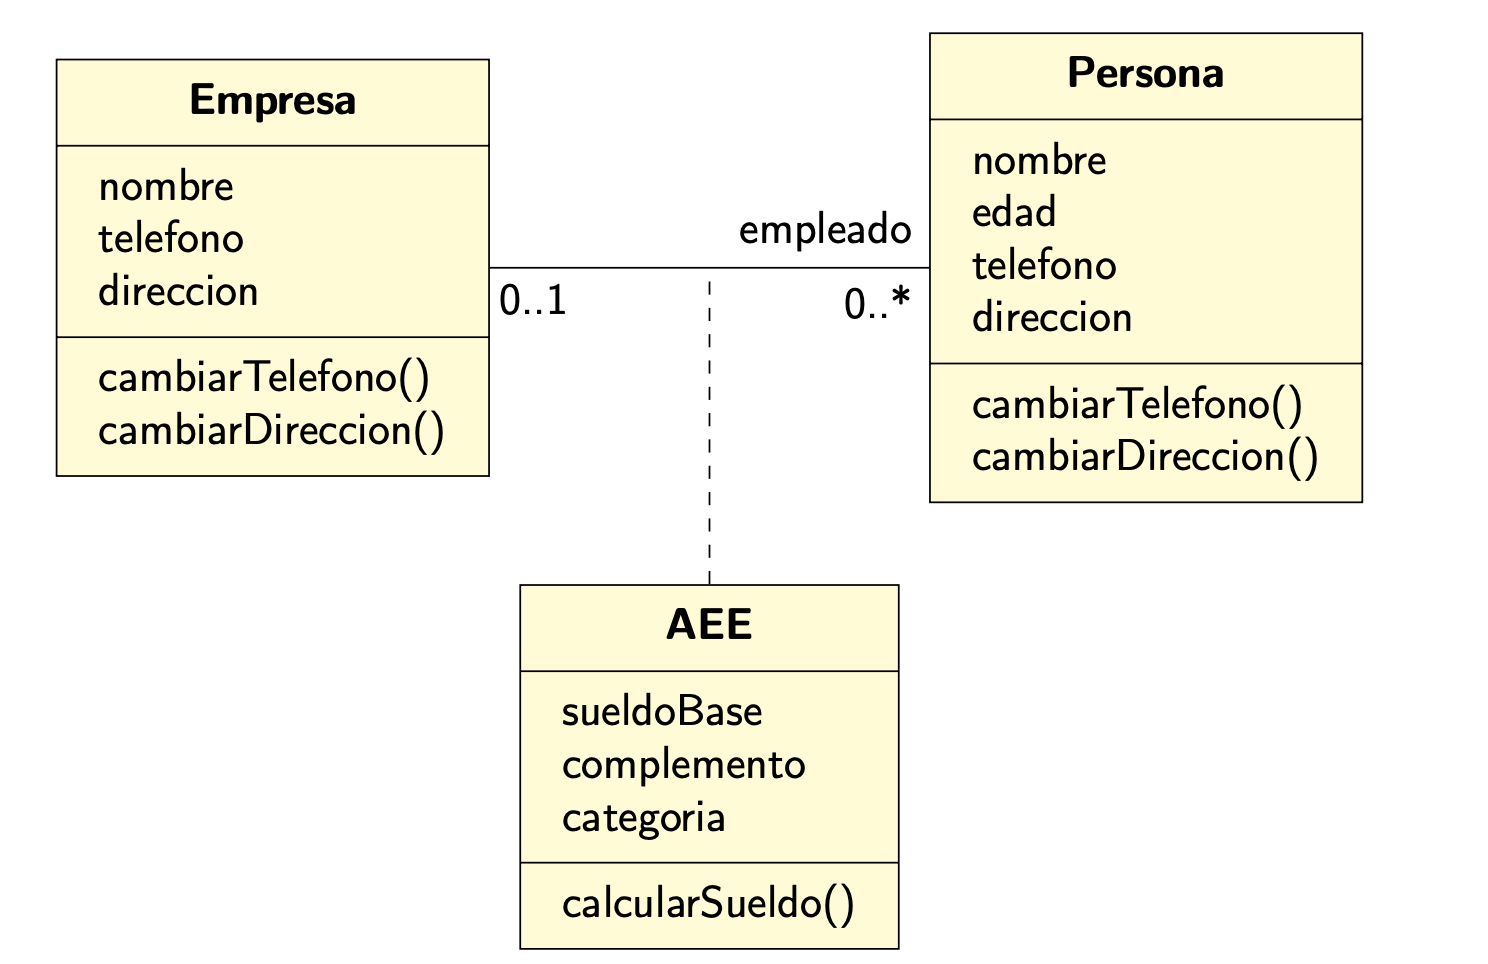
\includegraphics[width=\textwidth]{Imagenes/AClS.png}
    \caption{Asociación con Clase de Asociación}
\end{figure}
\begin{center}
	\begin{lstlisting}[frame=single]
class Empresa{};
class Persona{};
class Salario{};
class AEE{//clase de asociacion resultante
  public:
    void setA(Empresa&,Persona&,Salario&);
    void setB(Persona&,Empresa&,Salario&);
    const std::map<Persona*,Salario*>* getB(Empresa&)const;
    const std::map<Empresa*,Salario*>* getA(Persona&)const;
  private:
    typename std::map<Empresa*,std::map<Persona*,Salario*>>AD;
    typename std::map<Persona*,std::map<Empresa*,Salario*>>AI;
    AD ab;
    AI ba;
};
\end{lstlisting}
\end{center}
Si la multiplicidad en una de las dos clases es 0..1, podemos hacer uso de '\texttt{pair}' en vez de \texttt{map}.\\
En este caso, como empresa es 0..1, hacemos \texttt{std::map<Persona*,std::pair$<$Empresa*,Salario*$>$$>$* AI$;$}
\subsection{Implementación clase de asociación con 2 clases}

\begin{center}
	\begin{figure}[h]
	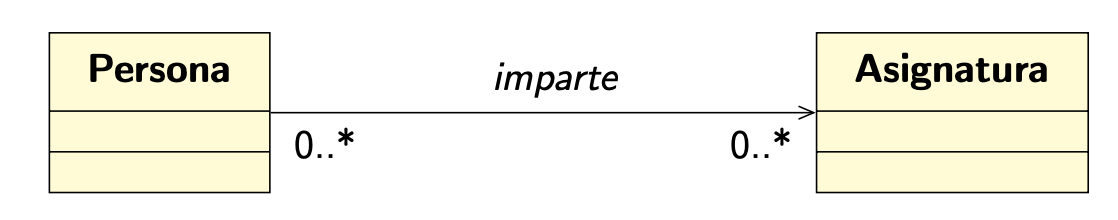
\includegraphics[width=\textwidth]{Imagenes/AClS2.png}
	\caption{Asociación muchos - muchos con Clase de Asociación}
\end{figure}
\end{center}
También es una alternativa para implementar la asociación entre dos clases, siempre y cuando la multiplicidad sea muchos - muchos o no tengamos el código fuente de ambas clases y no podamos incluir los métodos propios de la asociación.\vspace*{0,2cm}\\
Podemos crearnos una clase nueva, que representa la relación entre estas dos clases.
\begin{center}
	\begin{lstlisting}[frame=single]
class Persona{};
class Asignatura{};
class PersonaAsignatura{
  public:
	typedef std::multimap<Persona*,Asignatura*>AD;
	//otra manera -> typedef std::map<Persona*,std::set<Asignatura*>> AD;
	typedef std::multimap<Asignatura*,Persona*>AI;
	//typedef std::map<Asignatura*,std::set<Persona*>>AI;
	void setPersona(Persona&,Asignatura&);
	void setAsignatura(Asignatura&,Persona&);
	void getPersona(Asignatura&)const;
	void getAsignatura(Persona&)const;
	//std:set<Persona*>& getPersona(Asignatura&)const;
	//std::set<Asignatura*>& getAsignatura(Persona&)const;
  private:
  	///nos ayuda a insertar nuevos pares.
	bool esta(Persona&,Asignatura&)const;
	AD directa;
	AI inversa;
};
\end{lstlisting}
\end{center}
Para prevenir la inserción múltiple de valores a una clave tenemos 2 maneras:
\begin{enumerate}
	\item Si hacemos uso de \texttt{multimap} tenemos que declarar el método \texttt{esta()} para comprobar que dicho valor no está insertado.
	\item Podemos hacer uso de un \texttt {set} dentro de un \texttt{map}, haciendo que por cada clave puede haber un único conjunto de valores → \texttt{std::map<A*,std::set$<$B*$>$$>$Nombre$;$}\\

\end{enumerate}
\begin{center}
	\begin{lstlisting}[frame=single]
bool PersonaAsignatura::esta(Persona& p, Asignatura& a) const{ 
//std::pair<PersonaImparteAsignatura::ID,
//         PersonaImparteAsignatura::ID>
//         rango = directa.equal_range(&p);
auto rango = directa.equal_range(&p);//devuelve un rango <first,second>
for (PersonaImparteAsignatura::ID i = rango.first; i != rango.second; ++i)
    if (i->second == &a) return true;
  return false;
}
\end{lstlisting}
\end{center}
En el método \texttt {esta()} tenemos que buscar todas las ocurrencias de dicha clave, por tnato, \texttt{find} no nos sirve ya que nos devuelve la primera y necesitamos todas. Por tanto, usamos \texttt{equal\_range(&clave)}
 para poder obtener un rango (la primero y última ocurrencia que tiene esa clave).
Para poder obtener el conjunto de personas o de asignaturas mediante un set dentro de un map:
\begin{center}
	\begin{lstlisting}[frame=single]
std::set<Asignatura*> PersonaAsignatura::getAsignatura(Persona& p)const{
	auto i = directa.find(&p);
		if(i!=directa.end())return i->second; //*i.second;
	else return std::set<Asignatura*>();//devolvemos conjunto vacío.
}

std:set<Persona*> PersonaAsignatura::getPersona(Asignatura& a)const{
	auto i = inversa.find(&a);
	if(i!=inversa.end()) return i->second;
	else return std::set<Persona*>(); //devolvemos conjunto vacío.
}
\end{lstlisting}
\end{center}
\begin{quote}
	\textbf{La devolución del set que es un conjunto vacío lo va a realizar mediante movimiento, el conjunto devuelto normal será una copia.}
\end{quote}
\newpage
\subsection{Clase genérica de asociación con 2 clases}
\begin{center}
	\begin{lstlisting}[frame=single]
template <typename X, typename Y>
class AsociacionBidireccional{
public:
  void asocia(X& x, Y& y);
  void asocia(Y& y, X& x);
  std::set<Y*> asociados(X& x) const;
  std::set<X*> asociados(Y& y) const;
private:
  std::map<X*, std::set<Y*> > directa;
  std::map<Y*, std::set<X*> > inversa;
//-----Implementación de los métodos-----

// Asocia bidireccionalmente dos objetos .
template <typename X, typename Y>
void AsociacionBidireccional<X, Y>::asocia(X& x, Y& y){
    directa[&x].insert(&y);
    inversa[&y].insert(&x);
}
template <typename X, typename Y>
inline void AsociacionBidireccional<X, Y>::asocia(Y& y, X& x)
{ asocia(x, y); }

// Devuelve el conjunto de enlaces asociados a un objeto .
template <typename X, typename Y>
std::set<Y*> AsociacionBidireccional<X, Y>::asociados(X& x) const
{
  typename std::map<X*, std::set<Y*>>::
     const_iterator i = directa.find(&x);
  if (i != directa.end()) return i->second;
  else return std::set<Y*>();
}
template <typename X, typename Y>
std::set<X*> AsociacionBidireccional<X, Y>::asociados(Y& y) const
{
  typename std::map<Y*, std::set<X*>>::
     const_iterator i = inversa.find(&y);
  if (i != inversa.end()) return i->second;
  else return std::set<X*>();
}
\end{lstlisting}
\end{center}
\newpage
\subsection{Clase genérica de asociación con atributo de enlace}
\begin{center}
	\begin{lstlisting}[frame=single]
template <typename X, typename Y, typename Z> 
// X e Y: clases asociadas
// Z: clase de los atributos de enlace
class AsociacionBidireccional {
public:
  void asocia(X& x, Y& y, Z& z);
  void asocia(Y& y, X& x, Z& z);
  map<Y*, Z*> asociados(X& x) const;
  map<X*, Z*> asociados(Y& y) const;
private:
  map<X*, map<Y*, Z*> > directa;
  map<Y*, map<X*, Z*> > inversa;
};
//-----Implementacion de los métodos-----

// Asocia bidireccionalmente dos objetos .
template <typename X, typename Y, typename Z>
void AsociacionBidireccional<X, Y, Z>::asocia(X& x, Y& y, Z& z){
	//directa[&x][&y]=(&z); //permite modificar z
	directa[&x].insert(make_pair(&y, &z));
	//inversa[&y][&x]=(&z); //permite modificar z
	inversa[&y].insert(make_pair(&x, &z));
}
template <typename X, typename Y, typename Z> inline
void AsociacionBidireccional<X, Y, Z>::asocia(Y& y, X& x, Z& z)
 { asocia(x, y, z); }
 
// Devuelve el conjunto de enlaces asociados a un objeto .
template <typename X, typename Y, typename Z>
map<Y*,Z*> AsociacionBidireccional<X, Y, Z>::asociados(X& x) const
{
  map<X*, map<Y*, Z*>>::const_iterator i = directa.find(&x);
  if (i != directa.end()) return i->second; //por valor
  else return map<Y*, Z*>(); //diccionario vacío por movimiento
}
template <typename X, typename Y, typename Z>
map<X*,Z*> AsociacionBidireccional<X, Y, Z>::asociados(Y& y) const
{
  map<Y*, map<X*, Z*>>::const_iterator i = inversa.find(&y);
  if (i != inversa.end()) return i->second;
  else return map<X*, Z*>();//diccionario vacío por movimiento
}
\end{lstlisting}
\end{center}